\documentclass{article}
\usepackage[utf8]{inputenc}
% are all of these packages really necessary?
% no.
% i'm just too lazy to only grab the packages i want for a specific
% document, so i just glob all of my most commonly used packages together
% this is bad practice.
\usepackage{amsmath,amsthm,amssymb,amsfonts, fancyhdr, color, comment, graphicx, environ, mdframed, soul, calc, enumitem, mdframed, xcolor, geometry, empheq, mathtools, tikz, pgfplots, caption, subcaption, hyperref,multicol, esint}

\usetikzlibrary{external}
\tikzexternalize[prefix=tikz/,optimize command away=\includepdf]

%tikzpicture
\usepackage{tikz}
\usepackage{scalerel}
\usepackage{pict2e}
\usepackage{tkz-euclide}
\usetikzlibrary{calc}
\usetikzlibrary{patterns,arrows.meta}
\usetikzlibrary{shadows}
\usetikzlibrary{external}

%pgfplots
\usepackage{pgfplots}
\pgfplotsset{compat=newest}
\usepgfplotslibrary{statistics}
\usepgfplotslibrary{fillbetween}
\usepgfplotslibrary{polar}

\tikzset{external/export=true}
\pgfplotsset{
    standard/.style={
    axis line style = thick,
    trig format=rad,
    enlargelimits,
    axis x line=middle,
    axis y line=middle,
    enlarge x limits=0.15,
    enlarge y limits=0.15,
    every axis x label/.style={at={(current axis.right of origin)},anchor=north west},
    every axis y label/.style={at={(current axis.above origin)},anchor=south east}
    }
}
\newcommand*\widefbox[1]{\fbox{\hspace{2em}#1\hspace{2em}}}
% Command "alignedbox{}{}" for a box within an align environment
% Source: http://www.latex-community.org/forum/viewtopic.php?f=46&t=8144
\newlength\dlf  % Define a new measure, dlf
\newcommand\alignedbox[2]{
% Argument #1 = before & if there were no box (lhs)
% Argument #2 = after & if there were no box (rhs)
&  % Alignment sign of the line
{
\settowidth\dlf{$\displaystyle #1$}  
    % The width of \dlf is the width of the lhs, with a displaystyle font
\addtolength\dlf{\fboxsep+\fboxrule}  
    % Add to it the distance to the box, and the width of the line of the box
\hspace{-\dlf}  
    % Move everything dlf units to the left, so that & #1 #2 is aligned under #1 & #2
\boxed{#1 #2}
    % Put a box around lhs and rhs
}
}

\hypersetup{
    colorlinks=true,
    linkcolor=blue,
    filecolor=magenta,      
    urlcolor=cyan,
    pdftitle={Homework 23 Solutions},
    pdfpagemode=UseOutlines,
    bookmarksopen=true,
    pdfauthor={Christina Phan}
}
\newcommand{\lrp}[1]{\left( #1 \right)}
\newcommand{\abs}[1]{\left\vert #1 \right\vert}
\newcommand{\lra}[1]{\left\langle #1 \right\rangle}
\newcommand{\lrb}[1]{\left[ #1 \right]}
\newcommand{\norm}[1]{\left\lVert #1 \right\rVert}
\newcommand{\iintR}[0]{\iint\limits_{R}}
\renewcommand{\u}[0]{\mathbf{u}}
\renewcommand{\i}[0]{\mathbf{{i}}}
\renewcommand{\j}[0]{\mathbf{{j}}}
\renewcommand{\k}[0]{\mathbf{{k}}}
\newcommand{\T}[0]{\mathbf{T}}
\newcommand{\N}[0]{\mathbf{N}}
\newcommand{\B}[0]{\mathbf{B}}
\renewcommand{\r}[0]{\mathbf{r}}
\renewcommand{\a}[0]{\mathbf{a}}
\renewcommand{\v}[0]{\mathbf{v}}
\newcommand{\F}[0]{\mathbf{F}}
\newcommand{\G}[0]{\mathbf{G}}
\newcommand{\n}[0]{{\mathbf{n}}}
\newcommand{\eqq}[0]{\stackrel{?}{=}}
\renewcommand{\arraystretch}{1.25}

\geometry{letterpaper, portrait, margin=1in}
\renewcommand{\footrulewidth}{0.8pt}
\setlength\parindent{0pt}
\pagestyle{fancy}
\lhead{Christina Phan}
\rhead{MAT 21D} 
\chead{\textbf{Homework 23 Solutions}}

\newcommand{\Solution}{\textit{Solution}}
\pgfplotsset{compat=1.18}
\begin{document}

\phantomsection
\addcontentsline{toc}{section}{Problem 1 (Parts)}\textbf{Problem 1 (Parts)}

Find the divergence of the vector field:

\phantomsection
\addcontentsline{toc}{subsection}{1(a)}\textbf{(a)} $\F(x,y,z)=\lra{x\ln y, \ln z, z\ln x}$

\Solution

Recall that the divergence of a vector field is
\begin{equation*}
    \text{div }\F=\nabla \cdot \F=\lra{\frac{\partial }{\partial x},\frac{\partial }{\partial y},\frac{\partial }{\partial z}}\cdot \lra{M,N,P}=\frac{\partial}{\partial x}\lrp{M}+\frac{\partial}{\partial y}\lrp{N}+\frac{\partial}{\partial z}\lrp{P}
\end{equation*}
Since $\F(x,y,z)=\lra{x\ln y, \ln z, z\ln x}$,
\begin{align*}
  \text{div }\F&=\frac{\partial}{\partial x}(x\ln y) +\frac{\partial}{\partial y}(y \ln z) + \frac{\partial}{\partial z}(z \ln x)\\
  &=\lrp{\ln y }+ \lrp{\ln z }+ \lrp{\ln x}\\
  &=\boxed{\ln x + \ln y + \ln z}
\end{align*}

\phantomsection
\addcontentsline{toc}{subsection}{1(b)}\textbf{(b)} $\F(x,y,z)=\lra{\sin xy, \cos yz, \tan xz}$

\Solution

Recall that the divergence of a vector field is
\begin{equation*}
    \text{div }\F=\nabla \cdot \F=\lra{\frac{\partial }{\partial x},\frac{\partial }{\partial y},\frac{\partial }{\partial z}}\cdot \lra{M,N,P}=\frac{\partial}{\partial x}\lrp{M}+\frac{\partial}{\partial y}\lrp{N}+\frac{\partial}{\partial z}\lrp{P}
\end{equation*}
Since $\F(x,y,z)=\lra{\sin xy, \cos yz, \tan xz}$,
\begin{align*}
  \text{div }\F&=\frac{\partial}{\partial x}(\sin xy) +\frac{\partial}{\partial y}(\cos yz) + \frac{\partial}{\partial z}(\tan xz)\\
  &=\lrp{y\cos xy }+ \lrp{-z\sin yz}+\lrp{ x\sec^2 z}\\
  &=\boxed{x\sec^2 z + y\cos xy - z\sin yz}
\end{align*}

\phantomsection
\addcontentsline{toc}{subsection}{1(c)}\textbf{(c)} $\F=\nabla \times \G$, where the components of $\G$ have continuous second partial derivatives

\Solution

Recall that the divergence of a vector field is
\begin{equation*}
    \text{div }\F=\nabla \cdot \F=\lra{\frac{\partial }{\partial x},\frac{\partial }{\partial y},\frac{\partial }{\partial z}}\cdot \lra{M,N,P}=\frac{\partial}{\partial x}\lrp{M}+\frac{\partial}{\partial y}\lrp{N}+\frac{\partial}{\partial z}\lrp{P}
\end{equation*}

Let $\G=\lra{A,B,C}$ be a vector field where $A$, $B$, and $C$ have continuous second partial derivatives.

Since $\F=\nabla\times\G$,
\begin{align*}
   \F&=\nabla \times \G\\
   &=\begin{vmatrix}\i & \j & \k\\ \frac{\partial}{\partial x} & \frac{\partial}{\partial y}& \frac{\partial}{\partial z}\\ A & B & C\end{vmatrix}\\
    &=\Bigg(\frac{\partial }{\partial y}(C)-\frac{\partial }{\partial z}(B)\Bigg)\i-\Bigg(\frac{\partial}{\partial x}(C)-\frac{\partial}{\partial z}(A)\Bigg)\j+\Bigg(\frac{\partial}{\partial x}(B)-\frac{\partial}{\partial y}(A)\Bigg)\k\\
     &=\Bigg(\frac{\partial }{\partial y}(C)-\frac{\partial }{\partial z}(B)\Bigg)\i+\Bigg(-\frac{\partial}{\partial x}(C)+\frac{\partial}{\partial z}(A)\Bigg)\j+\Bigg(\frac{\partial}{\partial x}(B)-\frac{\partial}{\partial y}(A)\Bigg)\k\\
    &=\lra{\frac{\partial C}{\partial y}-\frac{\partial B}{\partial z}, -\frac{\partial C}{\partial x}+\frac{\partial A}{\partial z},\frac{\partial B}{\partial x}-\frac{\partial A}{\partial y}}
\end{align*}
Let's find the divergence of $\F = \displaystyle \lra{\frac{\partial C}{\partial y}-\frac{\partial B}{\partial z}, -\frac{\partial C}{\partial x}+\frac{\partial A}{\partial z},\frac{\partial B}{\partial x}-\frac{\partial A}{\partial y}}$.
\begin{align*}
    \text{div }\F&=\lra{\frac{\partial}{\partial x},\frac{\partial}{\partial y},\frac{\partial}{\partial z}}\cdot \lra{\frac{\partial C}{\partial y}-\frac{\partial B}{\partial z}, -\frac{\partial C}{\partial x}+\frac{\partial A}{\partial z},\frac{\partial B}{\partial x}-\frac{\partial A}{\partial y}}\\
    &=\frac{\partial }{\partial x}\lrp{ \frac{\partial C}{\partial y}-\frac{\partial B}{\partial z}}+\frac{\partial }{\partial y}\lrp{- \frac{\partial C}{\partial x}+\frac{\partial A}{\partial z}}+\frac{\partial }{\partial z}\lrp{ \frac{\partial B}{\partial x}-\frac{\partial A}{\partial y}}\\
    &=\lrp{\frac{\partial^2 C}{\partial x \partial y}- \frac{\partial ^2 B}{\partial x\partial z}}+\lrp{-\frac{\partial^2 C}{\partial y \partial x}+ \frac{\partial ^2 A}{\partial y\partial z}}+\lrp{\frac{\partial^2 B}{\partial z \partial x}- \frac{\partial ^2 A}{\partial z\partial y}}\\
    &= \lrp{\frac{\partial ^2 C}{\partial x \partial y}-\frac{\partial ^2 C}{\partial y \partial x}}+\lrp{-\frac{\partial^2 B}{\partial x\partial z}+\frac{\partial^2 B}{\partial z\partial x}}+\lrp{\frac{\partial ^2 A}{\partial y\partial z}-\frac{\partial^2 A}{\partial z\partial y}}\tag{rearrange}\\
    &=\lrp{0}+\lrp{0}+\lrp{0}\tag{mixed second partial derivatives are equal}\\
    &=\boxed{0}
\end{align*}
\phantomsection
\addcontentsline{toc}{section}{Problem 2 (Parts)}\textbf{Problem 2 (Parts)}

Use the Divergence Theorem to integrate $\F$ over the boundary of the region $D$:

\phantomsection
\addcontentsline{toc}{subsection}{2(a)}\textbf{(a)} $\F(x,y,z)=\lra{x^2,y^2,z^2}$, $D_1$, is the cube cut from the first octant by the planes $x=1$, $y=1$, and $z=1$; $D_2$ is the region cut from the cylinder $x^2+y^2=4$ by the planes $z=0$ and $z=1$.

\Solution


\phantomsection
\addcontentsline{toc}{subsubsection}{D1} $D_1$

Recall that by Divergence Theorem,
\begin{equation*}
    \oiint_S \F\cdot \n \,d\sigma = \iiint_D \nabla \cdot \F\,dV
\end{equation*}
Since $\F(x,y,z)=\lra{x^2,y^2,z^2}$,
\begin{align*}
    \nabla \cdot \F&=\lra{\frac{\partial }{\partial x},\frac{\partial }{\partial y},\frac{\partial }{\partial z}}\cdot \lra{x^2,y^2,z^2}\\
    &=\frac{\partial}{\partial x}\lrp{x^2}+\frac{\partial}{\partial y}\lrp{y^2}+\frac{\partial}{\partial z}\lrp{z^2}\\
    &=2x+2y+2z
\end{align*}
Let's find the bounds for $D$ in terms of $x$, $y$, and $z$.

Our lower and upper bounds for $z$ are $z=0$ and $z=1$, respectively.

Our lower and upper bounds for $y$ are $y=0$ and $y=1$, respectively.

Our lower and upper bounds for $x$ are $x=0$ and $x=1$, respectively.

Let's evaluate the integral.
\begin{align*}
 \oiint_S \F\cdot \n \,d\sigma &=   \iiint_D \nabla \cdot \F\,dV\\
 &=  \int_0^1 \int_0^1 \int_0^1 2x+2y+2z\,dz\,dy\,dx\\
    &=\int_0^1\int_0^1 \lrb{2xz+2yz+z^2}_0^1 \,dy\,dx\\
    &=\int_0^1 \int_0^1 2x + 2y + 1\,dy\,dx\\
    &=\int_0^1 \lrb{2xy+y^2+y}_0^1 \,dx\\
    &=\int_0^1 2x+1+1\,dx\\
    &=\lrb{x^2+x+x}_0^1\\
    &=1+1+1\\
    &=3
\end{align*}

\phantomsection
\addcontentsline{toc}{subsubsection}{D2} $D_2$

Recall that by Divergence Theorem,
\begin{equation*}
    \oiint_S \F\cdot \n \,d\sigma = \iiint_D \nabla \cdot \F\,dV
\end{equation*}
Since $\F(x,y,z)=\lra{x^2,y^2,z^2}$,
\begin{align*}
    \nabla \cdot \F&=\lra{\frac{\partial }{\partial x},\frac{\partial }{\partial y},\frac{\partial }{\partial z}}\cdot \lra{x^2,y^2,z^2}\\
    &=\frac{\partial}{\partial x}\lrp{x^2}+\frac{\partial}{\partial y}\lrp{y^2}+\frac{\partial}{\partial z}\lrp{z^2}\\
    &=2x+2y+2z
\end{align*}
Let's find the bounds for $D$ in terms of $x$, $y$, and $z$.

Our lower and upper bounds for $z$ are $z=0$ and $z=1$, respectively.

We can get our lower and upper bounds for $x$ and $y$ from $x^2+y^2=4$.

Graphically, the $xy$ region looks like a circle of radius $2$.
\begin{center}
\resizebox{3.5cm}{!}{
    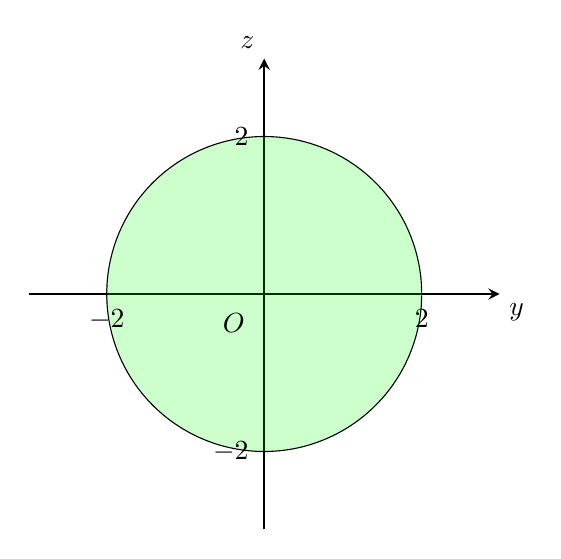
\begin{tikzpicture}
    \begin{axis}[standard,
            xtick={-2,2},
            ytick={-2,2},
            samples=1000,
            xlabel={$y$},
            ylabel={$z$},
          xmin=-2.3,
          xmax=2.3,          
          ymin=-2.3,
          ymax=2.3,
            x=1cm,
            y=1cm/1,
           ]

    \node[anchor=center,label=south west:$O$] at (axis cs:0,0){};
\addplot[name path=F,domain={-2:2}]{sqrt(4-x^2)};
\addplot[name path=G,domain={-2:2}]{-sqrt(4-x^2)};
\addplot[fill=green, fill opacity=0.2] fill between [of=F and G, soft clip={domain=-3:3}];
    \end{axis}
    \end{tikzpicture}
}
\end{center}
A circle... let's covert the $xy$ region into a polar region. Don't forget that we'll need to throw in our Jacobian $r$ into our integral.

Our lower and upper bounds for $r$ are $r=0$ and $r=2$, respectively.

Our lower and upper bounds for $\theta$ are $\theta=0$ and $\theta=2\pi$, respectively.

In polar, we know $x=r\cos\theta$, $y=r\sin\theta$, and $z=z$. Therefore,
\begin{equation*}
    \nabla \cdot \F=2x+2y+2z=2r\cos\theta+2r\sin\theta+2z
\end{equation*}
Let's evaluate the integral.
\begin{align*}
    \oiint_S\F\cdot\n\,d\sigma &= \iiint_D\nabla\cdot\F\,dV\\
    &=\int_0^{2\pi}\int_0^2 \int_0^1 \lrp{2r\cos\theta+2r\sin\theta + 2z}r\,dz\,dr\,d\theta\tag{don't forget our Jacobian $r$!}\\
    &=\int_0^{2\pi}\int_0^2 2r^2\cos\theta+2r^2\sin\theta+2rz\,dz\,dr\,d\theta\\
    &=\int_0^{2\pi}\int_0^2 \lrb{2r^2z\cos\theta+2r^2z\sin\theta+rz^2}_0^1\,dr\,d\theta\\
    &=\int_0^{2\pi}\int_0^2 2r^2\cos\theta + 2r^2\sin\theta + r\,dr\,d\theta\\
    &=\int_0^{2\pi}\lrb{\frac{2}{3}r^3\cos\theta+\frac{2}{3}r^3\sin\theta+\frac{1}{2}r^2}_0^2\,d\theta\\
    &=\int_0^{2\pi} \frac{2}{3}(2)^3\cos\theta+\frac{2}{3}(2)^3\sin\theta+\frac{1}{2}(2)^2\,d\theta\\
    &=\int_0^{2\pi} \frac{16}{3}\cos\theta+\frac{16}{3}\sin\theta + 2\,d\theta\tag{use a calculator}\\
    &=\lrb{\frac{16}{3}\sin\theta -\frac{16}{3}\cos\theta + 2\theta}_0^{2\pi}\\
    &=\lrp{\frac{16}{3}\sin2\pi-\frac{16}{3}\cos2\pi + 2(2\pi)}-\lrp{\frac{16}{3}\sin 0 -\frac{16}{3}\cos 0 + 2(0)}\\
    &=\lrp{0 - \frac{16}{3}+ 4\pi}-\lrp{0 - \frac{16}{3}+0}\\
    &=\lrp{-\frac{16}{3}+4\pi}- \lrp{-\frac{16}{3}}\\
    &=\boxed{4\pi}
\end{align*}
Our final answer is
\begin{subequations}
    \begin{empheq}[box=\widefbox]{align}
        D_1& :3\nonumber\\
       D_2& :4\pi\nonumber
    \end{empheq}
\end{subequations}

\phantomsection
\addcontentsline{toc}{subsection}{2(b)}\textbf{(b)} $\F(x,y,z)=\lra{x^2,-2xy,3xz}$, $D$ is the region cut from the first octant by the
sphere $x^2+y^2+z^2=4$

\Solution

Recall that by Divergence Theorem,
\begin{equation*}
    \oiint_S \F\cdot \n \,d\sigma = \iiint_D \nabla \cdot \F\,dV
\end{equation*}
Since $\F(x,y,z)=\lra{x^2,-2xy,3xz}$,
\begin{align*}
    \nabla \cdot \F&=\lra{\frac{\partial }{\partial x},\frac{\partial }{\partial y},\frac{\partial }{\partial z}}\cdot \lra{x^2,-2xy,3xz}\\
    &=\frac{\partial}{\partial x}\lrp{x^2}+\frac{\partial}{\partial y}\lrp{-2xy}+\frac{\partial}{\partial z}\lrp{3xz}\\
    &=\lrp{2x}+\lrp{-2x}+\lrp{3x}\\
    &=3x
\end{align*}
Let's find the bounds for $D$ in spherical coordinates since we have a (part of a) sphere as our region. Don't forget that since we're switching to spherical coordinates, we'll need to throw in our Jacobian $\rho^2\sin\phi$ into our integral. 

Since $x^2+y^2+z^2=4$, we have a sphere of radius $\sqrt{4}=2$.

Our lower and upper bounds for $\rho$ are $\rho=0$ and $\rho=2$, respectively.

Since we're \textit{only} in the first octant, our lower and upper bounds for $\phi$ are $\phi = 0$ and $\phi = \dfrac{\pi}{2}$, respectively.

Since we're \textit{only} in the first octant, our lower and upper bounds for $\theta$ are $\theta=0$ and $\theta=\dfrac{\pi}{2}$, respectively.
\begin{figure}[h]
\centering
\begin{minipage}{.5\textwidth}
  \centering
  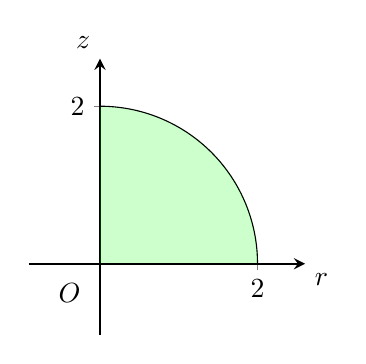
\begin{tikzpicture}
    \begin{axis}[standard,
            xtick={2},
            ytick={2},
            samples=1000,
            xlabel={$r$},
            ylabel={$z$},
            xmin=-0.5,xmax=2.2,
            ymin=-.5,ymax=2.2,
            x=1cm,
            y=1cm/1,
           ]
\node[anchor=center,label=south west:$O$] at (axis cs:0,0){};
\addplot[name path=F,domain={0:2}]{sqrt(4-x^2)};
\addplot[name path=G,domain={0:2}]{0};
\addplot[fill=green, fill opacity=0.2] fill between [of=F and G, soft clip={domain=0:2}];
    \end{axis}
    \end{tikzpicture}
  \caption*{front view}
  \label{fig:test2}
\end{minipage}%
\begin{minipage}{.5\textwidth}
  \centering
  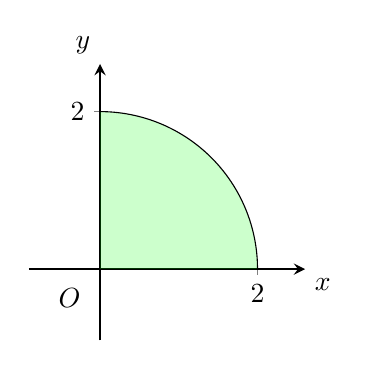
\begin{tikzpicture}
    \begin{axis}[standard,
            xtick={2},
            ytick={2},
            samples=1000,
            xlabel={$x$},
            ylabel={$y$},
            xmin=-.5,xmax=2.2,
            ymin=-.5,ymax=2.2,
            x=1cm,
            y=1cm/1,
           ]
\node[anchor=center,label=south west:$O$] at (axis cs:0,0){};
\addplot[name path=F,domain={0:2}]{sqrt(4-x^2)};
\addplot[name path=G,domain={0:2}]{0};
\addplot[fill=green, fill opacity=0.2] fill between [of=F and G, soft clip={domain=0:2}];
    \end{axis}
    \end{tikzpicture}
  \caption*{top view}
  \label{fig:test2}
\end{minipage}
\end{figure}

In spherical coordinates, we know $x=\rho\sin\phi\cos\theta$, $y=\rho\sin\phi\sin\theta$, and $z=\rho\cos\phi$. Therefore,
\begin{equation*}
    \nabla \cdot \F= 3x=3\rho\sin\phi\cos\theta
\end{equation*}
Let's evaluate the integral.
\begin{align*}
  \oiint_S \F\cdot \n\,d\sigma&=\iiint_D\nabla\cdot\F\,dV\\  &=\int_0^{\pi/2}\int_0^{\pi/2} \int_0^{2} \lrp{3\rho\sin\phi\cos\theta}\lrp{\rho^2\sin\phi}\,d\rho\,d\phi\,d\theta\tag{don't forget our Jacobian $\rho^2\sin\phi$!}\\
    &=\int_0^{\pi/2}\int_0^{\pi/2}\int_0^2 3\rho^3 \sin^2\phi\cos\theta\,d\rho\,d\phi\,d\theta\\
    &=\int_0^{\pi/2}\int_0^{\pi/2}\lrb{\frac{3}{4}\rho^4\sin^2\phi\cos\theta}_0^2\,d\phi\,d\theta\\
    &=\int_0^{\pi/2}\int_0^{\pi/2} \frac{3}{4}(2)^4\sin^2\phi\cos\theta\,d\phi\,d\theta\\
    &=\int_0^{\pi/2}\int_0^{\pi/2} 12\sin^2\phi\cos\theta\,d\phi\,d\theta\tag{use a calculator}\\
    &=\int_0^{\pi/2}\int_0^{\pi/2}12\lrp{\frac{1}{2}(1- \cos 2\phi)}\cos\theta\,d\phi\,d\theta\tag{$\sin^2\phi =\dfrac{1}{2}(1-\cos2\phi)$}\\
    &=\int_0^{\pi/2}\int_0^{\pi/2}6(1-\cos 2\phi)\cos\theta\,d\phi\,d\theta\\
    &=\int_0^{\pi/2}\int_0^{\pi/2} (6 - 6\cos 2\phi)\cos\theta\,d\phi\,d\theta\\
    &=\int_0^{\pi/2}\lrb{\lrp{6\phi - 3\sin 2\phi}\cos\theta}_0^{\pi/2}\,d\theta\\
    &=\int_0^{\pi/2} \lrp{\lrp{6\lrp{\frac{\pi}{2}}-3\sin 2\lrp{\frac{\pi}{2}}}\cos\theta}-\lrp{\lrp{6(0)-3\sin 2(0)}\cos \theta}\,d\theta\\
    &=\int_0^{\pi/2}\lrp{(3\pi - 3\sin \pi)\cos\theta}-\lrp{(0-3\sin 0)\cos\theta}\,d\theta\\
    &=\int_0^{\pi/2} \lrp{(3\pi)\cos\theta}- \lrp{(0)\cos\theta}\,d\theta\\
    &=\int_0^{\pi/2}3\pi\cos\theta \,d\theta\\
    &=\lrb{3\pi\sin\theta}_0^{\pi/2}\\
    &=\lrp{3\pi\sin\frac{\pi}{2}}-\lrp{3\pi\sin0}\\
    &=3\pi(1)-3\pi(0)\\
    &=\boxed{3\pi}
\end{align*}

\phantomsection
\addcontentsline{toc}{subsection}{2(c)}\textbf{(c)} $\F(x,y,z)=\lra{2xz,-xy,-z^2}$, $D$ is the wedge cut from the first octant by the plane $y+z=4$ and the elliptical cylinder $4x^2+y^2=16$

\Solution

Recall that by Divergence Theorem,
\begin{equation*}
    \oiint_S \F\cdot \n \,d\sigma = \iiint_D \nabla \cdot \F\,dV
\end{equation*}
Since $\F(x,y,z)=\lra{2xz,-xy,-z^2}$,
\begin{align*}
    \nabla \cdot \F&=\lra{\frac{\partial }{\partial x},\frac{\partial }{\partial y},\frac{\partial }{\partial z}}\cdot \lra{2xz,-xy,-z^2}\\
    &=\frac{\partial}{\partial x}\lrp{2xz}+\frac{\partial}{\partial y}\lrp{-xy}+\frac{\partial}{\partial z}\lrp{-z^2}\\
    &=\lrp{2xz}+\lrp{-xy}+\lrp{-z^2}\\
    &=\lrp{2z}+\lrp{-x}+\lrp{-2z}\\
    &=-x
\end{align*}
Let's find the bounds for $D$ in terms of $x$, $y$, and $z$.

Since we're in the first octant, our lower and upper bounds for $z$ are $z=0$ and $z=4-y$, respectively ($y+z=4\implies z=4-y$).

We can get our lower and upper bounds for $x$ and $y$ from  $4x^2+y^2=16$. 

Since $4x^2+y^2=16$, we know
\begin{align*}
    4x^2+y^2&=16\\
    y^2&=16-4x^2\\
    y&=\sqrt{16-4x^2}\tag{we're in first octant, $y\geq 0$}
\end{align*}
Our lower and upper bounds for $y$ are $y=0$ and $y=\sqrt{16-4x^2}$, respectively.

Graphically, $0\leq y\leq \sqrt{16-4x^2}$ looks like
\begin{center}
\resizebox{3.5cm}{!}{
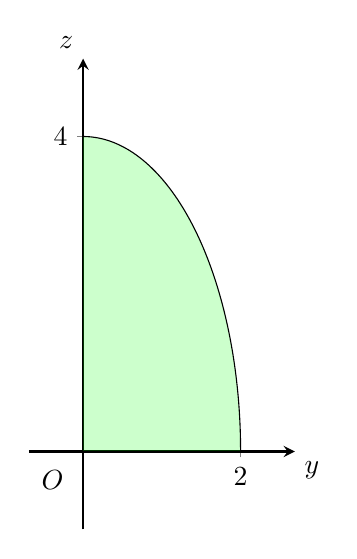
\begin{tikzpicture}
    \begin{axis}[standard,
            xtick={2},
            ytick={4},
            samples=1000,
            xlabel={$y$},
            ylabel={$z$},
          xmin=-.3,
          xmax=2.3,          
          ymin=-0.3,
          ymax=4.3,
            x=1cm,
            y=1cm/1,
           ]

    \node[anchor=center,label=south west:$O$] at (axis cs:0,0){};
\addplot[name path=F,domain={0:2}]{sqrt(16-4*x^2)};
\addplot[name path=G,domain={0:2}]{0};
\addplot[fill=green, fill opacity=0.2] fill between [of=F and G, soft clip={domain=0:2}];
    \end{axis}
    \end{tikzpicture}
}
\end{center}
Our lower and upper bounds for $x$ are $x=0$ and $x=2$, respectively. We could have also set $y=0$ to get $0=\sqrt{16-4x^2}$ and solve for $x$.

Let's evaluate the integral.
\begin{align*}
    \oiint_S \F\cdot \n\,d\sigma &=\iiint_D \nabla \cdot \F\,dV\\
    &=\int_0^2\int_0^{\sqrt{16-4x^2}}\int_0^{4-y}-x\,dz\,dy\,dx\\
    &=\int_0^2\int_0^{\sqrt{16-4x^2}}\lrb{-xz}_0^{4-y}\,dy\,dx\\
    &=\int_0^2\int_0^{\sqrt{16-4x^2}}-x(4-y)\,dy\,dx\\
    &=\int_0^2\int_0^{\sqrt{16-4x^2}}-4x+xy\,dy\,dx\\
    &=\int_0^2\lrb{-4xy+\frac{1}{2}xy^2}_0^{\sqrt{16-4x^2}}\,dx\\
    &=\int_0^2 {-4x\sqrt{16-4x^2}+\frac{1}{2}x\lrp{\sqrt{16-4x^2}}^2}\,dx\\
    &=\int_0^2 -4x\sqrt{16-4x^2}+\frac{1}{2}x(16-4x^2)\,dx\\
    &=\int_0^2 -4x\sqrt{16-4x^2}+ 8x - 2x^3\,dx\\
    &=\lrb{\frac{1}{3}(16-4x^2)^{3/2}+4x^2- \frac{1}{2}x^4}_0^2\\
    &=\lrp{\frac{1}{3}(16-4(2)^2)^{3/2}+4(2)^2-\frac{1}{2}(2)^4}-\lrp{\frac{1}{3}(16-4(0)^2)^{3/2}+4(0)^2-\frac{1}{2}(0)^4}\\
    &=\lrp{\frac{1}{3}(0)^{3/2}+16-8}-\lrp{\frac{1}{3}(16)^{3/2}+0-0}\\
    &=\lrp{16-8}-\lrp{\frac{1}{3}(64)}\\
    &=\boxed{-\frac{40}{3}}\tag{use a calculator}
\end{align*}

\phantomsection
\addcontentsline{toc}{subsection}{2(d)}\textbf{(d)} $\F(x,y,z)=\lra{5x^3+12xy^2,y^3+e^y\sin z, 5z^3+e^y\cos z}$, $D$ is the solid region between the spheres $x^2+y^2+z^2=1$ and $x^2+y^2+z^2=2$

\Solution

Recall that by Divergence Theorem,
\begin{equation*}
    \oiint_S \F\cdot \n \,d\sigma = \iiint_D \nabla \cdot \F\,dV
\end{equation*}
Since $\F(x,y,z)=\lra{5x^3+12xy^2,y^3+e^y\sin z, 5z^3+e^y\cos z}$,
\begin{align*}
    \nabla \cdot \F&=\lra{\frac{\partial }{\partial x},\frac{\partial }{\partial y},\frac{\partial }{\partial z}}\cdot \lra{5x^3+12xy^2,y^3+e^y\sin z, 5z^3+e^y\cos z}\\
    &=\frac{\partial}{\partial x}\lrp{5x^3+12xy^2}+\frac{\partial}{\partial y}\lrp{-y^3+e^y\sin z}+\frac{\partial}{\partial z}\lrp{5z^3+e^y\cos z}\\
    &=\lrp{15x^2+12y^2}+\lrp{3y^2+e^y\sin z}+\lrp{15z^2-e^y\sin z}\\
    &=15x^2+15y^2 + 15z^2\\
    &=15(x^2+y^2+z^2)
\end{align*}
Let's find the bounds for $D$ in spherical coordinates since we have two spheres as our region. Don't forget that since we're switching to spherical coordinates, we'll need to throw in our Jacobian $\rho^2\sin\phi$ into our integral.

Since $x^2+y^2+z^2=1$ and $x^2+y^2+z^2=2$, we have a sphere of radius $1$ and another sphere of radius $\sqrt{2}$.

Our lower and upper bounds for $\rho$ are $\rho = 1$ and $\rho = \sqrt{2}$, respectively.

Since we're going around the entire spheres, our lower and upper bounds for $\phi$ are $\phi=0$ and $\phi=\pi$. respectively.

Since we're going around the entire spheres, our lower and upper bounds for $\theta$ are $\theta=0$ and $\theta=2\pi$, respectively.


In spherical coordinates, we know $\rho^2 = x^2+y^2+z^2$. Therefore,
\begin{equation*}
    \nabla \cdot \F = 15(x^2+y^2+z^2)=15\rho^2
\end{equation*}
Let's evaluate the integral.
\begin{align*}
   \oiint_S \F\cdot \n\,d\sigma &=\iiint_D\nabla \cdot \F\,dV\\
   &=\int_0^{2\pi}\int_0^{\pi}\int_1^{\sqrt{2}} (15\rho^2)\lrp{\rho^2\sin\phi}\,d\rho\,d\phi\,d\theta\tag{don't forget our Jacobian $\rho^2\sin\phi$!}\\
    &=\int_0^{2\pi}\int_0^{\pi}\int_1^{\sqrt{2}} 15\rho^4\sin\phi\,d\rho\,d\phi\,d\theta\\
    &=\int_0^{2\pi}\int_0^\pi\lrb{3\rho^5\sin\phi}_1^{\sqrt{2}}\,d\phi\,d\theta\\
    &=\int_0^{2\pi}\int_0^\pi 3(\sqrt{2})^5\sin\phi - 3(1)^5\sin\phi\,d\phi\,d\theta\\
    &=\int_0^{2\pi}\int_0^{\pi} 12\sqrt{2}\sin\phi-3\sin\phi\,d\phi\,d\theta\tag{$(\sqrt{2})^5=(2^{4/2})(2^{1/2})=4\sqrt{2}$}\\
    &=\int_0^{2\pi}\int_0^{\pi}\lrp{12\sqrt{2}-3}\sin\phi\,d\phi\,d\theta\\
    &=\int_0^{2\pi}\lrb{-\lrp{12\sqrt{2}-3}\cos \phi}_0^{\pi}\,d\theta\\
    &=\int_0^{2\pi}\lrp{-\lrp{12\sqrt{2}-3}\cos\pi}-\lrp{-\lrp{12\sqrt{2}-3}\cos 0}\,d\theta\\
    &=\int_0^{2\pi}\lrp{12\sqrt{2}-3}-\lrp{-12\sqrt{2}+3}\,d\theta\\
    &=\int_0^{2\pi} 24\sqrt{2} - 6\,d\theta\\
    &=\lrb{\lrp{24\sqrt{2}-6}\theta}_0^{2\pi}\\
    &=\lrp{24\sqrt{2}-6}\lrp{2\pi}\\
    &=\boxed{\lrp{48\sqrt{2}-12}\pi}
\end{align*}

\phantomsection
\addcontentsline{toc}{subsection}{2(e)}\textbf{(e)} $\displaystyle\F(x,y,z)=\lra{\ln (x^2+y^2), -\frac{2z}{x}\tan^{-1}\frac{y}{x},z\sqrt{x^2+y^2}}$, $D$ is the ``thick-walled" cylinder $1\leq x^2+y^2\leq 2$, $-1 \leq z \leq 2$

\Solution

Recall that by Divergence Theorem,
\begin{equation*}
    \oiint_S \F\cdot \n \,d\sigma = \iiint_D \nabla \cdot \F\,dV
\end{equation*}
Since $\F(x,y,z)=\lra{\ln (x^2+y^2), -\frac{2z}{x}\tan^{-1}\frac{y}{x},z\sqrt{x^2+y^2}}$,
\begin{align*}
    \nabla \cdot \F&=\lra{\frac{\partial }{\partial x},\frac{\partial }{\partial y},\frac{\partial }{\partial z}}\cdot \lra{\ln (x^2+y^2), -\frac{2z}{x}\tan^{-1}\frac{y}{z},z\sqrt{x^2+y^2}}\\
    &=\frac{\partial}{\partial x}\lrp{\ln (x^2+y^2)}+\frac{\partial}{\partial y}\lrp{-\frac{2z}{x}\tan^{-1}\frac{y}{x}}+\frac{\partial}{\partial z}\lrp{z\sqrt{x^2+y^2}}\\
    &= \lrp{\frac{2x}{x^2+y^2}}+\lrp{-\frac{2z}{x}\lrp{\frac{\frac{1}{x}}{1+\frac{y^2}{x^2}}}}+\lrp{\sqrt{x^2+y^2}}\\
    &=\frac{2x}{x^2+y^2}-\frac{2z}{x^2\lrp{1+\frac{y^2}{x^2}}}+\sqrt{x^2+y^2}\\
    &=\frac{2x}{x^2+y^2}-\frac{2z}{x^2+y^2}+\sqrt{x^2+y^2}
\end{align*}
Let's find the bounds for $D$ in cylindrical coordinates since we have cylinders as our region. Don't forget that since we're switching to cylindrical coordinates, we'll need to throw in our Jacobian $r$ into our integral.


Since $-1 \leq z \leq 2$, our lower and upper bounds for $z$ are $z=-1$ and $z=2$, respectively.

Since $1\leq x^2+y^2\leq 2$ and $r^2=x^2+y^2$ in cylindrical coordinates, $1\leq r^2 \leq 2\implies 1\leq r\leq 2$.

Our lower and upper bounds for $r$ are $r=1$ and $r=\sqrt{2}$, respectively.

Since we're going around the entire cylinders, our lower and upper bounds for $\theta$ are $\theta=0$ and $\theta=2\pi$, respectively.
\begin{center}
\resizebox{3.5cm}{!}{
    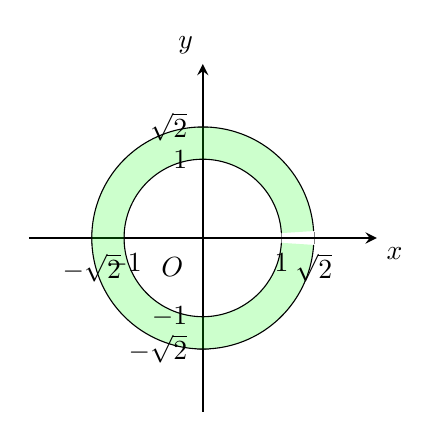
\begin{tikzpicture}
    \begin{axis}[standard,
            xtick={-1.41,-1,1,1.41},
            ytick={-1.41,-1,1,1.41},
            samples=1000,
            xlabel={$x$},
            ylabel={$y$},
            xmin=-1.7,xmax=1.7,
            ymin=-1.7,ymax=1.7,
            x=1cm,
            y=1cm/1,
            xticklabels={$-\sqrt{2}$,$-1$, $1$, $\sqrt{2}$},
            yticklabels={$-\sqrt{2}$,$-1$, $1$, $\sqrt{2}$}
           ]
\node[anchor=center,label=south west:$O$] at (axis cs:0,0){};
\addplot[name path=F,domain={-1.41:1.41}]{sqrt(1.41^2-x^2};
\addplot[name path=G,domain={-1:1}]{sqrt(1-x^2)};
\addplot[fill=green, fill opacity=0.2] fill between [of=F and G, soft clip={domain=-1.41:1.41}];
\addplot[name path=H,domain={-1.41:1.41}]{-sqrt(1.41^2-x^2};
\addplot[name path=I,domain={-1:1}]{-sqrt(1-x^2)};
\addplot[fill=green, fill opacity=0.2] fill between [of=H and I, soft clip={domain=-1.41:1.41}];
    \end{axis}
    \end{tikzpicture}
}
\end{center}
In cylindrical coordinates, we know $x=r\cos\theta$ and $r^2=x^2+y^2$. Therefore,
\begin{equation*}
    \nabla \cdot \F= \frac{2x}{x^2+y^2}-\frac{2z}{x^2+y^2}+\sqrt{x^2+y^2}=\frac{2r\cos\theta}{r^2}-\frac{2z}{r^2}+\sqrt{r^2}=\frac{2\cos\theta}{r}-\frac{2z}{r^2}+ r
\end{equation*}
Let's evaluate the integral.
\begin{align*}
    \oiint_S \F\cdot \n \,d\sigma&=\iiint_D \nabla \cdot \F\,dV\\
    &=\int_0^{2\pi}\int_1^{\sqrt{2}}\int_{-1}^2 \lrp{\frac{2\cos\theta}{r}-\frac{2z}{r^2}+ r}r\,dz\,dr\,d\theta\tag{don't forget our Jacobian $r$!}\\
    &=\int_0^{2\pi}\int_1^{\sqrt{2}}\int_{-1}^2 2\cos\theta-\frac{2z}{r}+r^2\,dz\,dr\,d\theta\\
    &=\int_0^{2\pi}\int_1^{\sqrt{2}}\lrb{2z\cos\theta-\frac{z^2}{r}+zr^2}_{-1}^2\,dr\,d\theta\\
    &=\int_0^{2\pi}\int_1^{\sqrt{2}} \lrp{2(2)\cos\theta-\frac{2^2}{r}+2r^2}-\lrp{2(-1)\cos\theta-\frac{(-1)^2}{r}+(-1)r^2}\,dr\,d\theta\\
    &=\int_0^{2\pi}\int_1^{\sqrt{2}} \lrp{4\cos\theta-\frac{4}{r}+2r^2 }-\lrp{-2\cos\theta -\frac{1}{r}-r^2}\,dr\,d\theta\\
    &=\int_0^{2\pi}\int_1^{\sqrt{2}} 6\cos\theta - \frac{3}{r}+3r^2\,dr\,d\theta\\
    &=\int_0^{2\pi}\lrb{6r\cos\theta-3\ln \left|r\right| + r^3}_1^{\sqrt{2}}\,d\theta\\
    &=\int_0^{2\pi}\lrp{6\sqrt{2}\cos\theta-3\ln \sqrt{2}+ (\sqrt{2})^3}-\lrp{6(1)\cos\theta-3\ln 1 + 1^3}\,d\theta\tag{$\sqrt{2},1> 0$}\\
    &=\int_0^{2\pi}\lrp{6\sqrt{2}\cos\theta-3\ln\sqrt{2}+2\sqrt{2}}-\lrp{6\cos\theta-0+1}\,d\theta\\
    &=\int_0^{2\pi}6\sqrt{2}\cos\theta -3\ln \sqrt{2}+2\sqrt{2}-6\cos\theta-1\,d\theta\\
    &=\lrb{6\sqrt{2}\sin\theta-3\ln\sqrt{2}\theta+2\sqrt{2}\theta-6\sin\theta-\theta}_0^{2\pi}\\
    &=\lrp{6\sqrt{2}\sin 2\pi -3\ln \sqrt{2}(2\pi)+2\sqrt{2}(2\pi)-6\sin2\pi - 2\pi}-\lrp{6\sqrt{2}\sin 0 -3\ln \sqrt{2}(0)+2\sqrt{2}(0)-6\sin 0 - 0}\\
    &=\lrp{0-6\ln\sqrt{2}\pi + 4\sqrt{2}\pi - 0 - 2\pi}-\lrp{0-0+0-0-0}\\
    &=-6\ln\sqrt{2}\pi + 4\sqrt{2}\pi-2\pi\\
    &=\boxed{\lrp{-6\ln \sqrt{2}+4\sqrt{2}-2}\pi}
\end{align*}
\phantomsection
\addcontentsline{toc}{section}{Problem 3 (Parts)}\textbf{Problem 3 (Parts)}

Recall the vector field $\F(x,y,z)=\lra{x,y,z}$ from problem 1 on Homework 22.

\phantomsection
\addcontentsline{toc}{subsection}{3(a)}\textbf{(a)} As suggest by the example in the lecture, show that the integral of $\F$ over any smooth closed surface $S$ is three times the volume of the region enclosed by $S$.

\Solution

Recall that by Divergence Theorem,
\begin{equation*}
    \oiint_S \F\cdot \n \,d\sigma = \iiint_D \nabla \cdot \F\,dV
\end{equation*}
Since $\F(x,y,z)=\lra{x,y,z}$,
\begin{align*}
    \nabla \cdot \F&=\lra{\frac{\partial }{\partial x},\frac{\partial }{\partial y},\frac{\partial }{\partial z}}\cdot \lra{x,y,z}\\
    &=\frac{\partial}{\partial x}\lrp{x}+\frac{\partial}{\partial y}\lrp{y}+\frac{\partial}{\partial z}\lrp{z}\\
    &= \lrp{1}+\lrp{1}+\lrp{1}\\
    &=3
\end{align*}
Let's evaluate the integral.
\begin{align*}
    \oiint_S \F\cdot \n \,d\sigma&=\iiint_D \nabla \cdot \F\,dV\\ &=\iiint_D 3\,dV\\
    &=3\iiint_D \,dV\tag{we can take constants out}\\
    &=3\times\text{volume of $S$}\tag{$\displaystyle \iiint_D \,dV$ is volume of region enclosed by $S$}
\end{align*}
\qed

\phantomsection
\addcontentsline{toc}{subsection}{3(b)}\textbf{(b)} Show that $\F$ is not orthogonal to the normal vector $\n$ at every point of $S$.

\Solution

If $\F$ is orthogonal to the normal vector $\n$ at every point of $S$, then $\F\cdot\n=0$ since the dot product of orthogonal vectors is $0$. Therefore, 
\begin{equation*}
    \oiint_S \F\cdot\n\,d\sigma = \iint_S 0\,d\sigma =0\tag{integral of $0$ is $0$}
\end{equation*}
However, we showed in 3(a) that $\displaystyle\oiint_S\F\cdot\n\,d\sigma$ is equal to three times the volume of the region enclosed by $S$. Since the volume of the region enclosed by $S$ is \textbf{not} $0$, $\displaystyle \oiint_S \F\cdot \n \neq 0$, so $\F$ \textbf{cannot} be orthogonal to the normal vector $\n$ at every point of $S$.

\qed

\addcontentsline{toc}{subsection}{3(c)}\textbf{(c)} Find a vector field with twice-differentiable components whose curl is $\F$ or prove
that no such field exists. (Using divergence makes this problem \textit{much} easier.)

\Solution

Let $\G=\lra{M,N,P}$ be a vector field with twice-differentiable components.

Since $\G=\lra{M,N,P}$,
\begin{align*}
   \text{curl }\G&= \nabla \times \mathbf{G} \\
   &=\begin{vmatrix}\i & \j & \k\\ \frac{\partial}{\partial x} & \frac{\partial}{\partial y}& \frac{\partial}{\partial z}\\ M & N & P\end{vmatrix}\\
    &=\Bigg(\frac{\partial }{\partial y}(P)-\frac{\partial }{\partial z}(N)\Bigg)\i-\Bigg(\frac{\partial}{\partial x}(P)-\frac{\partial}{\partial z}(M)\Bigg)\j+\Bigg(\frac{\partial}{\partial x}(N)-\frac{\partial}{\partial y}(M)\Bigg)\k\\
     &=\Bigg(\frac{\partial }{\partial y}(P)-\frac{\partial }{\partial z}(N)\Bigg)\i+\Bigg(-\frac{\partial}{\partial x}(P)+\frac{\partial}{\partial z}(M)\Bigg)\j+\Bigg(\frac{\partial}{\partial x}(N)-\frac{\partial}{\partial y}(M)\Bigg)\k\\
    &=\lra{\frac{\partial P}{\partial y}-\frac{\partial N}{\partial z}, -\frac{\partial P}{\partial x}+\frac{\partial M}{\partial z},\frac{\partial N}{\partial x}-\frac{\partial M}{\partial y}}
\end{align*}
Let's find the divergence of $\text{curl } \G$.
\begin{align*}
    \text{div }\lrp{\text{curl } \G}&=\lra{\frac{\partial}{\partial x},\frac{\partial}{\partial y},\frac{\partial}{\partial z}}\cdot \lra{\frac{\partial P}{\partial y}-\frac{\partial N}{\partial z}, -\frac{\partial P}{\partial x}+\frac{\partial M}{\partial z},\frac{\partial N}{\partial x}-\frac{\partial M}{\partial y}}\\
    &=\frac{\partial }{\partial x}\lrp{ \frac{\partial P}{\partial y}-\frac{\partial N}{\partial z}}+\frac{\partial }{\partial y}\lrp{- \frac{\partial P}{\partial x}+\frac{\partial M}{\partial z}}+\frac{\partial }{\partial z}\lrp{ \frac{\partial N}{\partial x}-\frac{\partial M}{\partial y}}\\
    &=\lrp{\frac{\partial^2 P}{\partial x \partial y}- \frac{\partial ^2 N}{\partial x\partial z}}+\lrp{-\frac{\partial^2 P}{\partial y \partial x}+ \frac{\partial ^2 M}{\partial y\partial z}}+\lrp{\frac{\partial^2 N}{\partial z \partial x}- \frac{\partial ^2 M}{\partial z\partial y}}\\
    &= \lrp{\frac{\partial ^2 P}{\partial x \partial y}-\frac{\partial ^2 P}{\partial y \partial x}}+\lrp{-\frac{\partial^2 N}{\partial x\partial z}+\frac{\partial^2 N}{\partial z\partial x}}+\lrp{\frac{\partial ^2 M}{\partial y\partial z}-\frac{\partial^2 M}{\partial z\partial y}}\tag{rearrange}\\
    &=\lrp{0}+\lrp{0}+\lrp{0}\tag{mixed second partial derivatives are equal}\\
    &=0
\end{align*}
If $\text{curl }\G = \F$, then $\text{div }\lrp{\text{curl } \G}=\text{div }\F$. However, we just showed that $\text{div }\lrp{\text{curl } \G}=0$ and we know from 3(a) that $\text{div }\F=3$. Since $0\neq 3$, we know $\F$ \textbf{cannot} be the curl of $\G$.

Therefore, there is no such field with twice-differentiable components whose curl is $\F$.

\qed

\phantomsection
\addcontentsline{toc}{section}{Problem 4}\textbf{Problem 4}

If $\F$ is a vector field with continuous first partial derivatives throughout a portion of
space containing a region $D$ bounded by a smooth closed surface $S$ such that $\norm{\F}\leq 1$,
can any bound be placed on $\displaystyle\iiint_D \nabla \cdot \F\,dV$?


\Solution

Recall that a dot product can be rewritten as
\begin{align*}
    \u \cdot \v &= \norm{\u}\norm{\v}\cos\theta\\
    \implies \left| \u \cdot \v\right| &= \left|\norm{\u}\norm{\v}\cos\theta\right|
\end{align*}
Recall that $\norm{\n}=1$ since $\n$ is a \textit{unit} normal vector.

Recall that $-1\leq \cos\theta\leq 1$, so $\left|\cos\theta\right|\leq 1$.

If $\norm{\F}\leq 1$, then
\begin{align*}
    \left|\F \cdot \n\right| &= \left|\norm{\F}\norm{\n}\cos\theta\right|\\
    &\leq \left|(1)(1)(1)\right|\\
    &\leq 1
\end{align*}
Recall that by Divergence Theorem,
\begin{align*}
    \iiint_D \nabla \cdot \F\,dV=\oiint_S \F\cdot \n \,d\sigma
\end{align*}
Since $\left|\F\cdot\n\right|\leq 1$,
\begin{align*}
     \iiint_D \nabla \cdot \F\,dV&=\oiint_S \F\cdot \n \,d\sigma\\
     &\leq \oiint_S \left|\F\cdot \n \right|\,d\sigma\\
     &\leq \oiint_S (1)\,d\sigma\\
     &\leq \oiint_S \,d\sigma\\
     &\leq \text{surface area of $S$}\tag{$\displaystyle\oiint_S\,d\sigma$ is just the surface area of $S$}
\end{align*}
Therefore, if $\norm{\F}\leq 1$, we know $\displaystyle \iint_D \nabla \cdot \F\,dV$ is at most the surface area of $S$.

\qed

\phantomsection
\addcontentsline{toc}{section}{"Problem 5"}\textbf{``Problem 5"}

be swag and go fill out your teaching evaluations at \texttt{eval.ucdavis.edu}!
\end{document}
